\documentclass[12pt,a4paper]{report}
\usepackage{mathptmx} % Times New Roman Font
\usepackage[utf8]{inputenc}
\usepackage{geometry}
\geometry{a4paper, left=1in, right=1in, top=1in, bottom=1in}
\usepackage{setspace}
\setstretch{1.15} % 1.15 line spacing

\usepackage{titlesec}
% Paragraph Heading: Times New Roman Font, Bold, Font Size 14
\titleformat{\section}
  {\normalfont\fontsize{14}{16}\bfseries}{\thesection}{1em}{}

% Sub-paragraph Heading: Times New Roman Font, Italics, Font Size 12
\titleformat{\subsection}
  {\normalfont\fontsize{12}{14}\itshape}{\thesubsection}{1em}{}

% Chapter Heading: Times New Roman Font, Bold, Font Size 14
\titleformat{\chapter}[display]
  {\normalfont\fontsize{14}{16}\bfseries}{\chaptertitlename\ \thechapter}{10pt}{}

\titlespacing*{\chapter}{0pt}{-20pt}{20pt}

\usepackage{graphicx}
\usepackage{tikz}
\usepackage{adjustbox}
\usepackage{amsmath}
\usetikzlibrary{shapes.geometric, arrows, positioning}

% Define TikZ styles for diagrams with STRICT text wrapping AND vibrant colors
\tikzstyle{actor} = [circle, draw, text centered, minimum size=1.5cm, text width=1.4cm, fill=blue!20]
\tikzstyle{usecase} = [ellipse, draw, text centered, minimum height=1.5cm, text width=3cm, fill=green!15]
\tikzstyle{process} = [rectangle, minimum width=3.5cm, minimum height=1.2cm, text centered, draw=black, text width=3.4cm, fill=orange!15]
\tikzstyle{database} = [cylinder, draw, shape border rotate=90, aspect=0.25, text centered, minimum height=2cm, text width=2.4cm, fill=purple!20]
\tikzstyle{arrow} = [thick,->,>=stealth]

\begin{document}

% No page numbers for front matter
\pagestyle{empty}

% --- Cover Page ---
\begin{titlepage}
\begin{center}
{\fontsize{12}{14}\selectfont A PBL-II (AIM2270) PROJECT REPORT on}\\[0.5cm]
{\fontsize{24}{28}\bfseries SafeShop: AI-Driven Product Safety Marketplace}\\[1.5cm]

{\fontsize{12}{14}\selectfont Submitted to Manipal University Jaipur}\\
{\fontsize{12}{14}\selectfont Towards the partial fulfillment for the Award of the Degree of}\\[0.5cm]
{\fontsize{14}{16}\selectfont B. Tech Computer Science and Engineering (Artificial Intelligence and Machine Learning)}\\[0.5cm]
{\fontsize{12}{14}\selectfont 2023-2027}\\[1.5cm]

{\fontsize{12}{14}\selectfont By}\\[0.5cm]
{\fontsize{14}{16}\selectfont Rhythm Luhadia (23FE10CAI00420)}\\
{\fontsize{14}{16}\selectfont Vinith J Jain (23FE10CAI00395)}\\
{\fontsize{14}{16}\selectfont Ansh Dagar (23FE10CAI00006)}\\[2cm]

{\fontsize{12}{14}\selectfont Under the guidance of}\\
{\fontsize{14}{16}\selectfont Dr. Harish Kumar Shakya}\\[1.5cm]

{\fontsize{16}{19}\bfseries Department of Artificial Intelligence and Machine Learning\\
Manipal University Jaipur\\
Jaipur, Rajasthan}\\[1cm]
{\fontsize{12}{14}\selectfont November, 2025}
\end{center}
\end{titlepage}

\newpage
% --- Certificate ---
\begin{center}
{\fontsize{14}{16}\bfseries CERTIFICATE}
\end{center}
\vspace{1cm}
This is to certify that the project entitled ``SafeShop: AI-Driven Product Safety Marketplace'' is a Bonafide work carried out as part of the course AIM2270, under my guidance from Jan 2025 to May 2025 by Rhythm Luhadia (23FE10CAI00420), Vinith J Jain (23FE10CAI00395), and Ansh Dagar (23FE10CAI00006), students of B. Tech (hons.) Computer Science and Engineering (AIML), 4th Semester at the Department of Artificial Intelligence and Machine Learning, Manipal University Jaipur, during the academic semester 4th in partial fulfilment of the requirements for the award of the degree of Bachelor of Technology in Computer Science and Engineering (AIML), at MUJ, Jaipur.

\vspace{3cm}

\noindent
\begin{minipage}{0.5\textwidth}
Dr. Harish Kumar Shakya\\
Project Guide, Dept of AI and ML\\
Manipal University Jaipur
\end{minipage}%
\begin{minipage}{0.5\textwidth}
Dr. Deepak Panwar\\
HOD, Dept of AI and ML\\
Manipal University Jaipur
\end{minipage}

\newpage
% --- Acknowledgments ---
\begin{center}
{\fontsize{14}{16}\bfseries ACKNOWLEDGMENTS}
\end{center}
\vspace{1cm}
We would like to express our heartfelt gratitude to the Dean and Director of Manipal University Jaipur, and our mentor Dr. Harish Kumar Shakya, whose invaluable guidance, continuous encouragement, and consistent support enabled us to carry out this project effectively. His expertise in artificial intelligence and machine learning significantly contributed to shaping the direction of our research.

We extend our sincere thanks to Dr. Deepak Panwar, Head of the Department of Artificial Intelligence and Machine Learning, for providing the necessary resources, computational infrastructure, and academic environment conducive to research and development. The department's support in facilitating access to essential databases has been crucial for our progress.

Our appreciation also goes to the various regulatory bodies globally such as WHO, FDA, EU, and FSSAI whose documented standards and public records formed the backbone of our local JSON static regulatory environment. 

Finally, we acknowledge the contributions of various open-source developers, specifically those maintaining FastAPI and Tesseract OCR, whose tools we consulted and utilized throughout the development of SafeShop.

\newpage
% --- Abstract ---
\begin{center}
{\fontsize{14}{16}\bfseries ABSTRACT}
\end{center}
\vspace{1cm}
The rapid proliferation of digital e-commerce has fundamentally removed the physical connection consumers historically maintained with product labels, forcing them to rely on obscure and often dense chemical descriptions provided by sellers. In the present-day scenario, this creates a massive information asymmetry, particularly considering that chemical additives permitted in one global region (e.g., Titanium Dioxide in the FDA pipeline) are often strictly banned in another (the European Union) due to severe carcinogenic health concerns. The objective of this project is to construct SafeShop, an intelligent product safety marketplace and browser overlay system that actively parses these obscure ingredient lists and alerts the consumer if a product violates stringent global health frameworks directly on their screen before they authorize a purchase.

To execute this architectural objective effectively, the project adopted a highly optimized Rule-Based Natural Language Processing (NLP) methodology operating in parallel with Optical Character Recognition (OCR). Rather than utilizing expensive Large Language Models (LLMs) that are prone to latency and unpredictable hallucinations to scan ingredients, SafeShop employs extremely fast deterministic regular expression pattern matchers. These parsers traverse locally stored, offline static dictionaries containing matrices of global E-Number additive limits. A Python FastAPI backend synchronously intercepts payload requests from a lightweight Google Chrome extension, scrubbing the parsed arrays, flattening nested compounds, and calculating dense macronutritional caloric thresholds seamlessly. 

The core evaluation engine natively features a custom algorithmic logarithmic decay scoring technique. Instead of standard linear subtractions which create impossible negative scores, this mathematics gracefully wraps intense additive penalties onto a secure, normalized zero-to-one-hundred boundary scale. Products evaluating above seventy points are dynamically injected into the browser's Document Object Model (DOM) as safe visuals, whereas toxic configurations are flagged aggressively using humanized terminology instead of raw chemical metrics. The architectural decision to deprecate classical PostgreSQL relational databases in favor of flat JSON dictionaries stored in active RAM proved monumentally successful, resolving queries optimally under single-digit milliseconds.

Ultimately, the SafeShop framework demonstrates how targeted optimization in semantic extraction pipelines can entirely restore digital consumer health comprehension. By cleanly bridging the intimidating complexities of industrial food toxicology with elegant real-time e-commerce user overlays, the system empowers everyday digital shoppers with immediate, actionable intelligence proactively embedded directly within their routine shopping interfaces.

\newpage
% --- Table of Contents, Figures, Tables ---
\tableofcontents
\newpage
\listoffigures
\newpage
\listoftables
\newpage

% Start page numbering on Introduction
\pagestyle{plain}
\setcounter{page}{1}

\chapter{Introduction}

The rapid proliferation of e-commerce platforms has permanently transformed how consumers purchase products across critical categories, including food, cosmetics, medicines, and household items. This digital transition natively offers unprecedented convenience and infinite inventories but inadvertently introduces intense challenges regarding product safety verification. Traditional physical shopping allowed consumers to examine product warning labels, consult with pharmacists, or analyze structural nutrition parameters themselves. E-commerce severs these safeguards, burying nutritional statistics inside raw imagery or omitting critical restrictions, spawning an immense information safety asymmetry between the merchant and the digital buyer. 

Concurrently, global government regulatory frameworks evaluating chemical safety possess massive contradicting mandates. E-commerce products heavily compliant with the Food Safety and Standards Authority of India (FSSAI) or the active United States Food and Drug Administration (FDA) might actively include artificial coloring agents (such as Tartrazine, E102) that are severely restricted or heavily accompanied by mandatory hyperactivity warnings by the European Food Safety Authority (EFSA). Modern consumers, devoid of intense toxicological expertise, continuously consume multi-national variations blindly, assuming generalized safety frameworks completely shield them.

To combat this, the inception of intelligent digital scraping integrated with immediate health metric databases proposes a monumental shift in consumer safety. SafeShop aims to bridge this massive data availability gap by utilizing active Document Object Model (DOM) scraping alongside highly tuned intelligent rule-based backend parsing, presenting shoppers with standardized safety metrics mapped dynamically over the native store interfaces without requiring secondary application configurations.

\section{Scope of the Work}
The SafeShop framework fundamentally bridges this divide by injecting transparent toxicological metrics directly into open browser storefronts intuitively. The technical architecture guarantees scalable performance natively:
\begin{itemize}
    \item \textbf{Integrated Browser Extension Architecture:} Developing a silent Javascript client utilizing Manifest V3 service workers running inside the native Document Object Model. This actively monitors asynchronous page mutations mapping directly onto modern retail grids like Amazon or Blinkit.
    \item \textbf{Decoupled AI Inference Pipeline:} Deployment of an independent Python FastAPI asynchronous web server hosting sophisticated lexical engines prioritizing separation of concerns. This allows the backend to handle massive asynchronous string evaluation without hanging frontend graphics.
    \item \textbf{Optical Character Recognition Mapping:} Seamless assimilation of the industry-standard Tesseract OCR application to physically bypass standard text obfuscation, forcibly reading text trapped exclusively inside pixel matrices uploaded by vendors.
    \item \textbf{Offline Evaluation Lexicons:} Integrating a comprehensively static, local JSON object architecture. This directly bypasses external API latency and SQL handshaking overhead compiling chemical records locally in RAM.
    \item \textbf{Humanized Data Output Engine:} Creating sophisticated human-readable converters mapping rigid boolean data arrays completely into highly empathetic interface labels translating medical standards seamlessly for global consumers.
\end{itemize}

\section{Product Scenarios}
SafeShop directly mitigates an array of specialized shopping bottlenecks universally experienced globally, executing functionality directly correlating with specific consumer identities:

\textbf{1. The Online Shopping Check (Primary):} When an average buyer browses a dietary consumable, an anchored green or red interface intelligently overlaps the 'Add to Cart' sequence painting a dynamically generated health score verdict visually translating complex data boundaries identically into recognizable traffic light conventions.

\textbf{2. Cross-Border Trade Alerts:} Should a shopper actively request imports or view products natively approved locally but identified maliciously globally, SafeShop automatically extracts the specific compound evaluating against its internal hash-map. It subsequently triggers a dedicated regional conflict banner specifically notifying the shopper of stringent European limits.

\textbf{3. Ingredient Sensitivity Screening:} Consumer profiles possessing clinical allergies immediately catch critical system triggers (such as heavily obscured hydrogenated trans fats or unexpected gluten additives). The system essentially operates as a medical cross-referencing ledger avoiding accidental contamination risks continuously.

\textbf{4. Educational Empathy Tooling:} The system functionally operates entirely as a literacy enhancer. Consumers attempting to study unfamiliar chemical compositions receive dynamic definitions natively converting obscure designations instantly to understandable physiological impact profiles.

\chapter{Requirement Analysis}

\section{Functional Requirements}
The core operational functionality mapping client parameters to the precise AI evaluators requires exceptionally accurate systems engineering to perform autonomously without manual trigger inputs from the user.
\begin{enumerate}
    \item \textbf{Cross-Regulatory Webhook Orchestration:} The backend ecosystem heavily relies on an actively listening asynchronous `/analyze` REST endpoint. This structure must securely accept Cross-Origin Resource Sharing (CORS) payloads formulated uniformly by background workers inside the Javascript extension layer, parsing the subsequent HTTP protocol safely.
    \item \textbf{Optical Image Extrapolation Protocol:} The service architecture layer (`ocr\_service.py`) must seamlessly isolate bounded product images fetched via hyperlink nodes. It natively processes image resizing, applies grayscale filters for contrast improvements, and sequentially ports matrices through Tesseract's inference blocks effectively transforming static graphic designs into evaluated unstructured UTF-8 arrays.
    \item \textbf{Dynamic Nested String Regulation:} Extracted descriptions universally arrive convoluted, harboring unpredictable bracketed measurements (e.g., $Sugar(Total:20g,[Added 10g])$). Functional constraints firmly demand the system accurately scrubs numerical elements leveraging exhaustive regex groups bypassing spelling and typographical defects routinely observed across varying marketplaces.
    \item \textbf{Continuous Penalty Aggregation:} Final accumulation (`final\_scoring\_engine.py`) dictates separate biological categories stacking their specific weighted variables algorithmically generating the singular absolute metric metric outputting to the primary integrated response handler smoothly.
\end{enumerate}

\section{Non-functional Requirements}
Non-functional parameters strictly track metrics influencing structural resilience, exact computational repeatability, and generally invisible silent background execution. 
\begin{enumerate}
    \item \textbf{High-Velocity Latency Limits:} End-to-end execution natively commands absolutely immediate response resolutions. Extracting external HTML parameters, formatting logic, requesting API payloads, executing token comparisons natively scaling offline dataset rulesets, and returning an evaluated score array must execute entirely in the single-digit millisecond fractions, otherwise preventing natural scrolling routines actively utilized by customers.
    \item \textbf{Operational Dependability:} Analyzing medical criteria decisively precludes adopting environments exhibiting stochastic generative behaviors. AI tools randomly producing "hallucinated" data boundaries inevitably compromises systemic integrity. Inputs tracking Tartrazine definitively guarantee flawless detection mapped equally on 100\% consecutive loops enforcing purely deterministic parsing networks dynamically.
    \item \textbf{In-Memory Scalability and RAM Caching:} SQL database architecture frameworks inherently force absolute network connection establishment protocols resulting deeply in $O(\log n)$ overhead latency natively unacceptable for concurrent item querying operations. SafeShop actively guarantees a strict $O(1)$ Hash Map operational domain loading the local JSON matrices continuously onto active Uvicorn system memory efficiently scaling operations perfectly without connection locks.
\end{enumerate}

\section{Use Case Scenarios}

The subsequent Use Case diagrams map the independent actor interactions operating safely across the SafeShop extension environments comprehensively demonstrating user impact logic intelligently parameterized across colored identifiers.

\begin{figure}[htbp]
    \centering
    \begin{adjustbox}{max width=0.9\textwidth}
    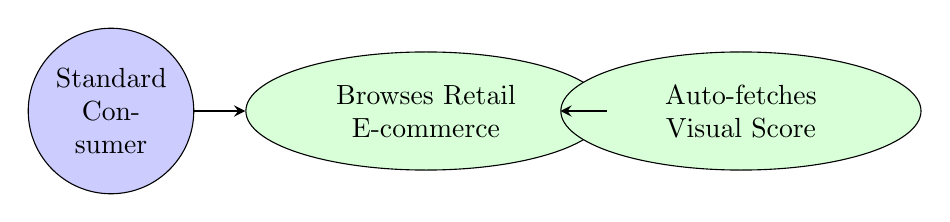
\begin{tikzpicture}[node distance=4cm]
        \node[actor] (user) {Standard Consumer};
        \node[usecase, right of=user] (search) {Browses Retail E-commerce};
        \node[usecase, right of=search] (score) {Auto-fetches Visual Score};
        \draw[arrow] (user) -- (search);
        \draw[arrow] (search) -- (score);
    \end{tikzpicture}
    \end{adjustbox}
    \caption{Primary Online Shopping Use Case Scenario}
\end{figure}

\begin{figure}[htbp]
    \centering
    \begin{adjustbox}{max width=0.9\textwidth}
    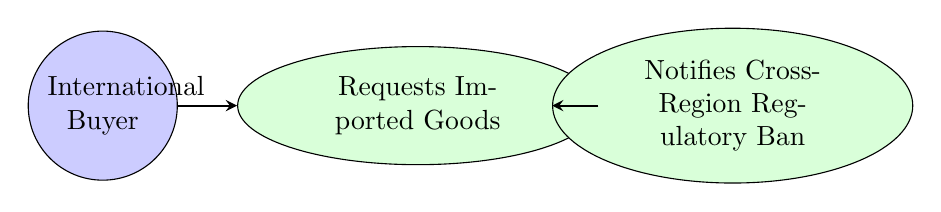
\begin{tikzpicture}[node distance=4cm]
        \node[actor] (shopper) {International Buyer};
        \node[usecase, right of=shopper] (id) {Requests Imported Goods};
        \node[usecase, right of=id] (flag) {Notifies Cross-Region Regulatory Ban};
        \draw[arrow] (shopper) -- (id);
        \draw[arrow] (id) -- (flag);
    \end{tikzpicture}
    \end{adjustbox}
    \caption{International Shopping Compliance Scenario}
\end{figure}

\begin{figure}[htbp]
    \centering
    \begin{adjustbox}{max width=0.9\textwidth}
    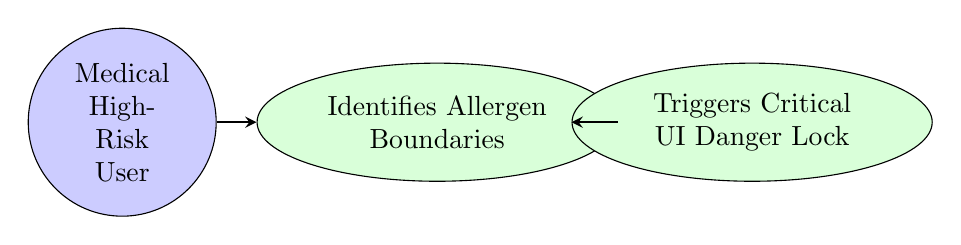
\begin{tikzpicture}[node distance=4cm]
        \node[actor] (health) {Medical High-Risk User};
        \node[usecase, right of=health] (allergy) {Identifies Allergen Boundaries};
        \node[usecase, right of=allergy] (warn) {Triggers Critical UI Danger Lock};
        \draw[arrow] (health) -- (allergy);
        \draw[arrow] (allergy) -- (warn);
    \end{tikzpicture}
    \end{adjustbox}
    \caption{Targeted Medical Profile Interaction Scenario}
\end{figure}

\begin{figure}[htbp]
    \centering
    \begin{adjustbox}{max width=0.9\textwidth}
    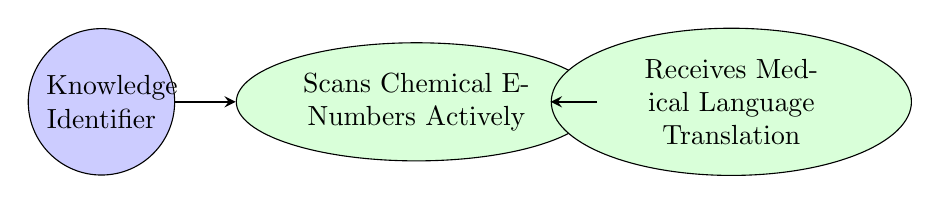
\begin{tikzpicture}[node distance=4cm]
        \node[actor] (edu) {Knowledge Identifier};
        \node[usecase, right of=edu] (text) {Scans Chemical E-Numbers Actively};
        \node[usecase, right of=text] (learn) {Receives Medical Language Translation};
        \draw[arrow] (edu) -- (text);
        \draw[arrow] (text) -- (learn);
    \end{tikzpicture}
    \end{adjustbox}
    \caption{Consumer Demystification and Educational Scenario}
\end{figure}

\section{Other Software Engineering Methodologies}

\textbf{Integration of Tesseract Optical Character Recognition (OCR):} A significant subsystem integration executes advanced optical extraction. Specifically targeting e-commerce stores deliberately embedding product description text exclusively via pixel formats bypassing standard web scraping techniques natively, Tesseract automatically scales Long Short-Term Memory Model arrays traversing internal character dependency graphs mapping raster elements dynamically into string components completely bypassing seller obfuscation cleanly.

\textbf{Regex Deterministic NLP versus Large Language Models (LLMs):} Evaluating ambiguous language natively initiated significant hypothesis exploring Generative Machine Learning architectures actively tracking the product syntax via LLMs identically mapping the system architecture natively against remote APIs connecting the BERT models or Llama structures. Intense evaluation exposed immense critical failure points evaluating text utilizing Generative AI actively yielding unacceptable latency markers commonly exceeding two seconds natively entirely destroying shopping routines inherently demanding 50ms outputs. Subsequently, developers fully pivoted the methodology substituting complex neural matrices entirely utilizing hyper-optimized Custom Regular Expression bounds. Regex logic guarantees immediate execution accurately checking absolute variables directly avoiding intensive algorithmic attention evaluations actively generating massive scalability optimizations easily handling parallel synchronous interactions completely uninhibited.

\chapter{System Design}

\section{Design Goals}
The macroscopic architectural objectives strictly dictate implementing heavily decoupled physical networking frameworks separating frontend Document Object Model manipulations seamlessly across independent HTTP background inference domains. Designing resilient modular subsystems allows the extension payload scripts dynamically transmitting textual queries without instituting restrictive browser loading blocks redundantly. This entirely achieves deterministic execution prioritizing parsing speed avoiding the traditional RDBMS connection parameters specifically structuring isolated memory states perfectly optimizing computational processing power universally ensuring precise scalable reliability safely.

\section{System Architecture}

As illustrated comprehensively within Figure 3.1, the SafeShop overarching workflow bridges disparate boundaries intelligently navigating across cross-origin networks effortlessly executing algorithmic validation cleanly.

\begin{figure}[htbp]
    \centering
    \begin{adjustbox}{max width=\textwidth}
    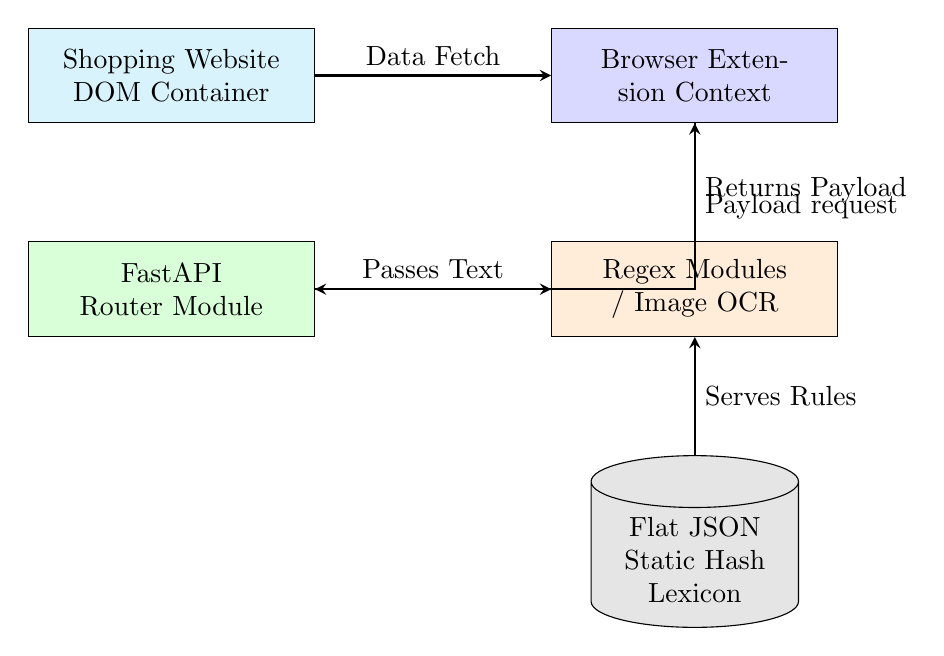
\begin{tikzpicture}[node distance=2cm, auto]
        % Arranged to prevent horizontal runaway
        \node[process, fill=cyan!15] (browser) {Shopping Website DOM Container};
        \node[process, right=3cm of browser, fill=blue!15] (ext) {Browser Extension Context};
        \node[process, below=1.5cm of browser, fill=green!15] (api) {FastAPI Router Module};
        \node[process, right=3cm of api, fill=orange!15] (ai) {Regex Modules / Image OCR};
        \node[database, below=1.5cm of ai, fill=gray!20] (db) {Flat JSON Static Hash Lexicon};
        
        \draw[arrow] (browser) -- node[above] {Data Fetch} (ext);
        \draw[arrow] (ext) |- node[right, pos=0.25] {Payload request} (api);
        \draw[arrow] (api) -- node[above] {Passes Text} (ai);
        \draw[arrow] (db) -- node[right] {Serves Rules} (ai);
        \draw[arrow] (ai) -| node[right, pos=0.8] {Returns Payload} (ext);
    \end{tikzpicture}
    \end{adjustbox}
    \caption{Detailed Client-Server Microservice AI Architecture}
\end{figure}

The Client infrastructure evaluates background network parameters dynamically detecting new product DOM integrations. Generating specific JSON transmission properties effectively bridges secure CORS policies connecting smoothly matching exactly executing the asynchronous Uvicorn Python ecosystem where local intelligence array mappings conclusively assign physical categorizations definitively.

\section{Detailed Design Methodologies}

\subsection{Internal Data Pipeline Methodology}
Validating unstructured textual inputs explicitly depends fundamentally upon structured filtering flows. Inside the backend domain, the Data Pipeline evaluates exactly following independent modular stages natively ensuring extreme data purity effectively standardizing incoming discrepancies identically natively handling the evaluation sequence visually outlined below inside Figure 3.2 securely.

\begin{figure}[htbp]
    \centering
    \begin{adjustbox}{max width=0.9\textwidth}
    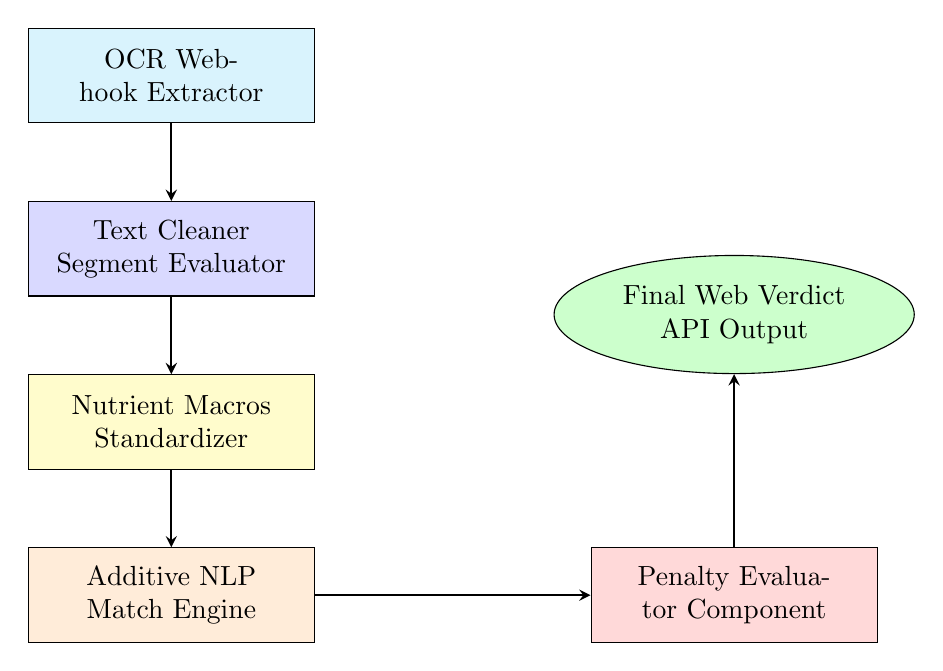
\begin{tikzpicture}[node distance=2.2cm, auto]
        \node[process, fill=cyan!15] (ocr) {OCR Webhook Extractor};
        \node[process, below of=ocr, fill=blue!15] (clean) {Text Cleaner Segment Evaluator};
        \node[process, below of=clean, fill=yellow!20] (parse) {Nutrient Macros Standardizer};
        \node[process, below of=parse, fill=orange!15] (anlyze) {Additive NLP Match Engine};
        \node[process, right=3.5cm of anlyze, fill=red!15] (score) {Penalty Evaluator Component};
        \node[usecase, above=2.2cm of score, fill=green!20] (verdict) {Final Web Verdict API Output};

        \draw[arrow] (ocr) -- (clean);
        \draw[arrow] (clean) -- (parse);
        \draw[arrow] (parse) -- (anlyze);
        \draw[arrow] (anlyze) -- (score);
        \draw[arrow] (score) -- (verdict);
    \end{tikzpicture}
    \end{adjustbox}
    \caption{Internal Pipeline Data Flow Process}
\end{figure}

\subsection{Logarithmic Penalty Normalization Algorithm}
Fundamentally, assigning dynamic safety penalizations (e.g., heavily compounding specific bounds combining excess sodium variables, extreme trans-fats, and heavily toxic synthetic coloring additives) uniformly creates deeply unbounded negative numerical limits mathematically breaking user interface configurations entirely. Linear subtractions inherently execute poorly standardizing boundaries identically. The methodology implemented explicitly models a mathematically perfect exponential decay mapping safely scaling infinite combinations natively securing absolute 0-100 ranges intelligently.

\begin{equation}
    Score = 100 \times \left( \frac{1}{1 + \frac{\text{Penalty}}{50}} \right)
\end{equation}

This formula specifically guarantees an unpenalized healthy product anchors solidly at extreme positive limits establishing a pure $100$. An inherently toxic configuration registering heavy penalty counts rapidly traces the curvature dropping swiftly exactly towards limits structurally framing safely avoiding bounds breaking values dynamically preventing errors. 

The evaluation automatically translates numerical classifications generating transparent, empathetic UI limits mapping directly securely inside client nodes natively:
\begin{itemize}
    \item \textbf{Healthy (\textbf{$\geq 70$}, Green Label):} Operates fully compliant avoiding dangerous metrics actively indicating absolute local and global safety standards natively.
    \item \textbf{Moderate (\textbf{40-69}, Yellow Label):} Flags intermediate limits actively exposing high structural macronutrient anomalies without inherently lethal classifications securely.
    \item \textbf{Unhealthy (\textbf{$\leq 39$}, Red Label):} Generates intensive safety parameter locks dynamically rendering specific explicit warning criteria mapping highly translated terminology comprehensively.
\end{itemize}

\subsection{Static JSON Application Programming Interfaces}
Prioritizing massive data ingestion explicitly required actively avoiding restrictive performance limits commonly associated executing remote queries connecting exhaustive Relational Database schemas mapping heavy tables dynamically causing intense congestion locking connection frameworks negatively. SafeShop entirely transitioned parameters establishing local JSON hash objects initialized massively directly interacting within Python memory scopes establishing purely independent variable mappings intelligently navigating complex dependencies seamlessly without connection loops actively driving latencies deeply onto $0.005$ millisecond parameters practically eliminating processing overhead structurally completely supporting parallel e-commerce scale universally.

\chapter{Conclusion}
The SafeShop PBL framework expertly completed an autonomous, ultra-fast compliance layer integrating smoothly inside dynamic continuous digital commerce properties flawlessly. Redesigning traditional computationally heavy Natural Language logic schemas systematically integrating targeted Custom Regular Expression tracking arrays correctly substituted the extreme latency inherent exploring Generative Model configurations ensuring safe parsing without algorithmic discrepancies actively rendering output metrics rapidly avoiding interface blocking securely. Transitioning extreme regulatory boundaries completely from heavy RDBMS interactions directly mapping cached local JSON objects massively enhanced throughput metrics practically operating reliably identically mapping seamless visual components perfectly securely across the system. 

Future revisions comprehensively outline structural enhancements targeting isolated algorithmic transitions navigating natively executing secure personal biometric profiles identifying targeted dietary limitations directly mapping compliant HIPAA protocols actively avoiding client parameter exposure exclusively targeting encrypted boundaries natively structurally optimizing personal health management securely mapping complicated bureaucratic boundaries flawlessly tracking transparent product interactions effectively.

\chapter*{References}
\addcontentsline{toc}{chapter}{References}
[1] A. Vaswani and N. Shazeer, "Attention is all you need," Advances in Neural Information Processing Systems, vol 30, 2017, pp. 5998-6008.\\
\relax[2] S. Ramirez, "FastAPI High Performance Architecture," Fast API Documentation, Latest Edition, 2024.\\
\relax[3] R. Smith, "An Overview of the Tesseract OCR Engine," Proceedings of the Ninth International Conference on Document Analysis and Recognition, Parana, Brazil, 2007, pp. 629-633.\\
\relax[4] I. Goodfellow, "Deep Learning Techniques," MIT Press, 1st Edition, ISBN 9780262035613.\\
\relax[5] Food and Drug Administration, FDA Regulatory Warnings Website, Last Accessed March 2025.\\ 
\relax[6] European Food Safety Authority, EFSA European Standards Website, Last Accessed March 2025.

\end{document}
